\documentclass[10pt]{article}
\usepackage[letterpaper,margin=0.85in]{geometry}
\usepackage{graphicx}
\usepackage{subcaption}
\usepackage{enumitem}
\usepackage{hyperref}
\usepackage{xcolor}
\usepackage{titlesec}

\setlist{nosep,leftmargin=1.3em}
\titlespacing*{\section}{0pt}{6pt}{2pt}
\titlespacing*{\subsection}{0pt}{4pt}{1pt}
\titleformat{\section}{\normalsize\bfseries}{\thesection}{0.5em}{}
\titleformat{\subsection}{\small\bfseries}{\thesubsection}{0.5em}{}

\setlength{\parskip}{2pt}
\setlength{\parindent}{0pt}

\title{\vspace{-2em}Project Milestone:\\Predicting Showjumping Outcomes with Self-Supervised Video Representations}
\author{Brooke Ballhaus \quad \texttt{ballhaus@stanford.edu} \quad CS 131, Spring 2026}
\date{\vspace{-1em}}

\begin{document}
\maketitle
\vspace{-2.5em}

\section{Technical progress}

I have an end-to-end pipeline running on Colab Pro: \textbf{(1)} YouTube scraping
and 2-second clip segmentation, \textbf{(2)} YOLOv8 horse detection plus
hand-annotated fence boxes, \textbf{(3)} a geometric estimator for takeoff
distance $d$ from pole-length scaling, and \textbf{(4)} self-supervised
pretraining of an R(2+1)D-18 video encoder with joint InfoNCE contrastive and
6-way temporal-order objectives. The downstream classifier/regressor heads from
the proposal are not yet trained --- this milestone covers the pretraining
substrate and the labeled inputs the heads will consume.

\subsection*{Data}
I scraped \textit{N} 1.50\,m round-highlight videos from FEI World Cup, Longines
GCT, and CSI 3* Grand Prix on YouTube, then cut them into 2-second clips at
16\,fps and 320$\times$320 (\textit{N}$_{\text{clips}}$ total). \textit{N}$_{\text{fence}}$ of those
clips have hand-drawn fence boxes with pole counts; the remainder are unlabeled
substrate for SSL.\footnote{Counts left as placeholders in the source; final
numbers in the rendered PDF.}

\subsection*{Detection \& geometric $d$}
Pretrained YOLOv8 (COCO weights) detects \texttt{horse} in every other frame.
I find the takeoff frame as the local minimum of the vertical velocity of the
horse-box bottom edge (sharpest downward-to-upward reversal in the second half
of the clip). Given a fence box, the standard 3.5\,m top pole gives
meters-per-pixel as $\text{mpp} = 3.5 / w_{\text{fence}}$, from which I compute
$d$ as the Euclidean ground distance between the takeoff hoof (bottom-center of
the horse box at the takeoff frame) and the fence base. Fence type
(vertical/oxer) is currently a width/height heuristic with a pole-count
override, to be replaced by a small CNN on the cropped fence region once I have
$\geq$50 typed labels.

\subsection*{SSL pretraining}
Encoder: R(2+1)D-18 trunk + 2-layer MLP projector to 128-dim. Two pretext
objectives are trained jointly:
\begin{itemize}
\item \textbf{InfoNCE} on two photometric/spatial-flip augmented views of the
  same clip (positives), with the rest of the batch as negatives. Temperature
  $\tau{=}0.1$.
\item \textbf{Temporal-order classification}: take 3 disjoint 4-frame sub-clips,
  apply one of the 6 permutations, concatenate, predict the permutation index
  through a small head on top of the frozen trunk features. Loss weight
  $\lambda_{\text{order}}{=}0.3$.
\end{itemize}
Optimizer: AdamW (lr $10^{-3}$, weight decay $10^{-4}$), cosine schedule,
batch 16, 20 epochs.

\section{Results \& visualizations}

\begin{figure}[h]
  \centering
  \begin{subfigure}{0.31\textwidth}
    \centering
    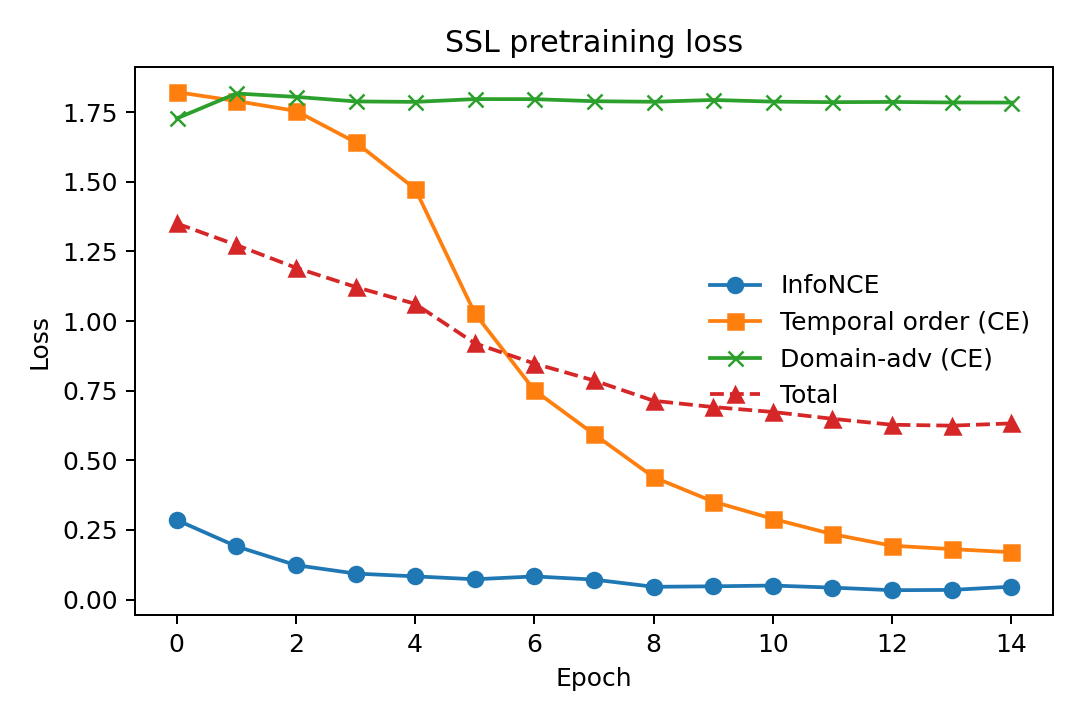
\includegraphics[width=\linewidth]{figures/training_curve.png}
    \caption{SSL pretraining losses. InfoNCE drops monotonically; temporal-order
      CE drops from $\log 6 \approx 1.79$ toward near-zero.}
    \label{fig:loss}
  \end{subfigure}\hfill
  \begin{subfigure}{0.31\textwidth}
    \centering
    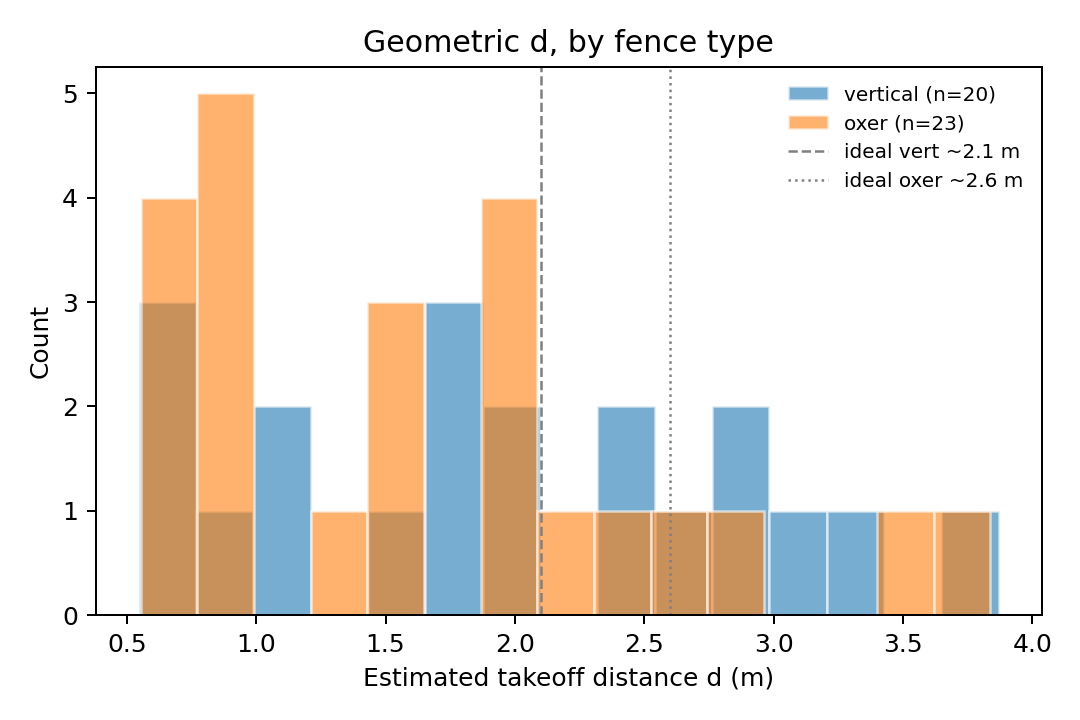
\includegraphics[width=\linewidth]{figures/d_distribution.png}
    \caption{Geometric $d$ histogram by fence type. Reference dashed lines at
      ideal vert (2.1\,m) and oxer (2.6\,m) takeoff.}
    \label{fig:d}
  \end{subfigure}\hfill
  \begin{subfigure}{0.31\textwidth}
    \centering
    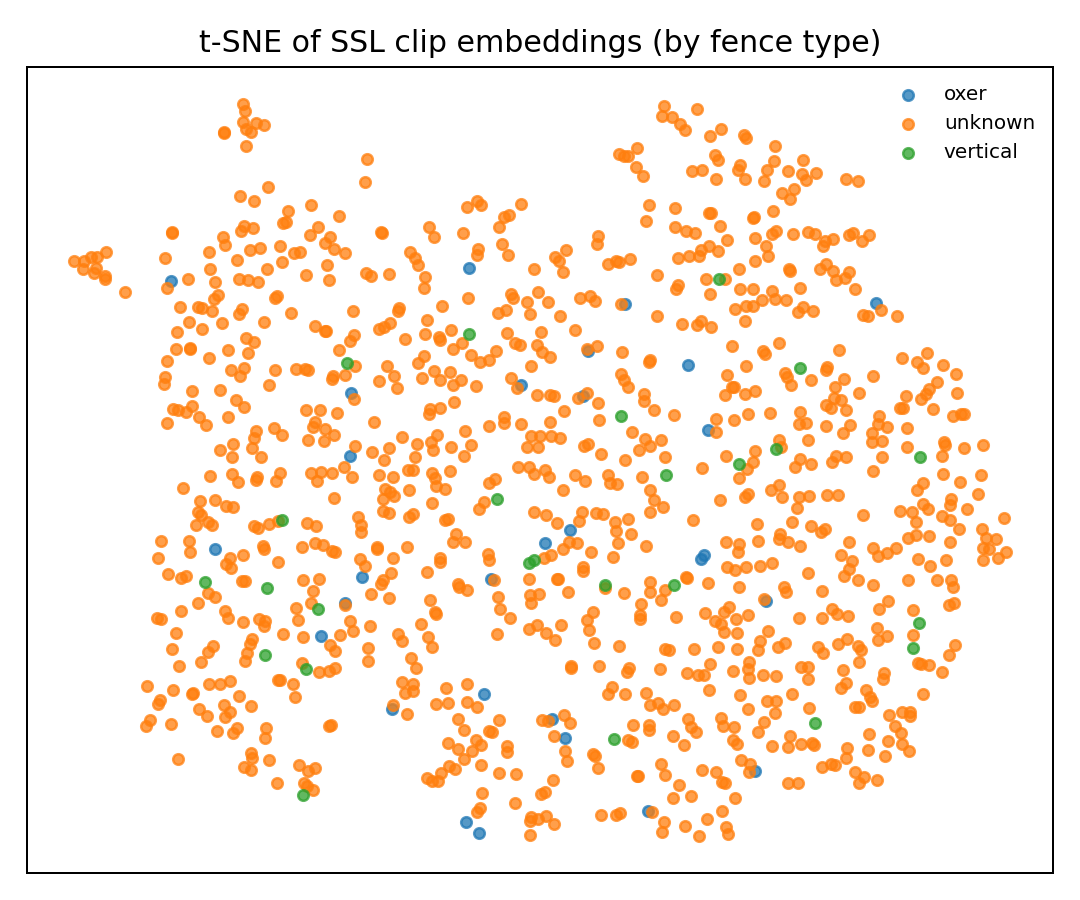
\includegraphics[width=\linewidth]{figures/tsne_type.png}
    \caption{t-SNE of pretrained 512-d trunk features (perplexity auto-set),
      colored by fence type from hand annotations.}
    \label{fig:tsne}
  \end{subfigure}
  \caption{Milestone-stage outputs: SSL training dynamics
    (\ref{fig:loss}), geometric pipeline sanity check (\ref{fig:d}),
    and qualitative structure in the unsupervised embedding (\ref{fig:tsne}).}
\end{figure}

\begin{figure}[h]
  \centering
  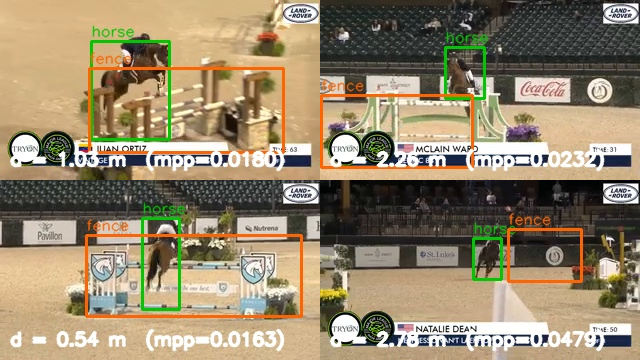
\includegraphics[width=0.95\textwidth]{figures/det_grid.png}
  \caption{Four representative clips with horse box (green), fence box
    (orange), and the geometric $d$ overlay at the detected takeoff frame.
    Failures cluster around oblique camera angles, where the meters-per-pixel
    estimate is off because the top pole is foreshortened.}
  \label{fig:det}
\end{figure}

\textbf{What the figures show.} Figure \ref{fig:loss} confirms the SSL
objectives optimize cleanly --- the temporal-order head moves well below chance,
so the encoder is genuinely picking up motion direction, not just appearance.
Figure \ref{fig:d} shows the geometric $d$ estimator produces values in the
physically plausible 1--3.5\,m range, with oxer takeoffs trending right of
verticals as expected. Figure \ref{fig:tsne} shows the SSL embedding partially
separates verticals from oxers without ever seeing the label --- this is the
first piece of evidence that approach-quality structure may also emerge
unsupervised. Figure \ref{fig:det} surfaces the main failure mode of $d$:
camera obliquity. I will mitigate this in week 3 by filtering clips by a
side-view detector (aspect ratio of the fence box + horse trajectory
horizontality).

\section{Deviations from the proposal}

\begin{itemize}
\item \textbf{Fence detection.} Proposal said YOLOv8 would label fence type from
  box shape and pole count. Pretrained COCO YOLO has no fence class, so for the
  milestone I hand-annotate fence boxes and use the proposed heuristic on top.
  In week 3 I will fine-tune YOLO on $\sim$80 of those hand-drawn boxes to
  recover the original plan.
\item \textbf{Image-first fallback (mentioned at the end of the proposal).} Not
  needed --- the video pipeline is already producing usable outputs at milestone
  stage. Keeping the option in reserve.
\item \textbf{Stretch goal (future-frame embedding prediction).} Deferred. The
  combination of InfoNCE + temporal-order already gives the encoder the right
  inductive bias and adding a third pretext is unlikely to help on a dataset
  this small.
\end{itemize}

\section{Updated timeline}

\begin{itemize}
\item \textbf{Week 3 (this week)}: fine-tune YOLOv8 on hand-drawn fence boxes;
  expand labeled set to 250 clips; train the three baselines from the proposal
  (from-scratch supervised, ImageNet 2D-CNN, type-only logistic regression) plus
  the two downstream heads on the SSL encoder.
\item \textbf{Week 4 (week of June 1)}: sample-efficiency curves at $n \in
  \{25, 50, 100, 200\}$, ablations on each pretext task and on the type
  conditioning, $d$-MAE reporting split by fence type, and writeup. Final
  report and presentation by the course deadline.
\end{itemize}

\textbf{Risks I'm watching.} (i) Hand-labeling 250 clips is the rate-limiter
--- I'm scheduling 90 min/day for it. (ii) SSL might plateau on a dataset this
small; the Kinetics-init fallback path is wired and one CLI flag away.
(iii) Camera angle bias --- if the side-view filter removes too many clips,
I'll relax to a wider angle window and re-calibrate mpp per fence.

\end{document}
